\documentclass[tikz,border=10pt]{standalone}
\usetikzlibrary{calc,angles,quotes}

\begin{document}
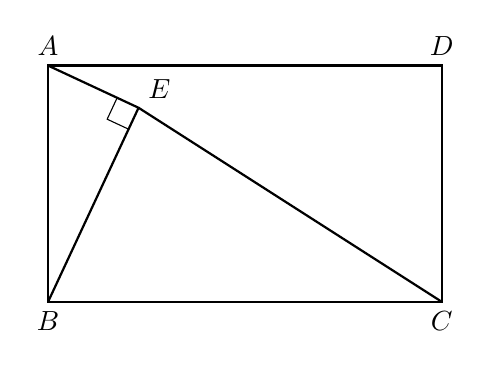
\begin{tikzpicture}
    % 1. 定义矩形顶点 (基于比例设定)
    \coordinate (B) at (0,0);
    \coordinate (A) at (0,3);
    \coordinate (D) at (5,3);
    \coordinate (C) at (5,0);
    
    % 2. 定义圆心 O (AB的中点)
    \coordinate (O) at (0,1.5);
    
    % 3. 绘制矩形
    \draw[thick] (A) -- (D) -- (C) -- (B) -- cycle;
    
    
    % 5. 定义点 E (在圆上，需满足BE perp AE)
    % 这里取一个合适的角度 theta，使得 E 在圆周上且 AE 垂直于 BE
    \def\ang{40} 
    \coordinate (E) at ($(O) + ({1.5*cos(\ang)}, {1.5*sin(\ang)})$);
    
    % 6. 绘制线段
    \draw[thick] (A) -- (E) -- (B);
    \draw[thick] (C) -- (E);

    
    % 7. 特殊点标注
    \node[above] at (A) {$A$};
    \node[below] at (B) {$B$};
    \node[below] at (C) {$C$};
    \node[above] at (D) {$D$};
    \node[above right] at (E) {$E$};

    % 8. 绘制直角标记
    \pic[draw, angle radius=3mm] {right angle = A--E--B};
    
\end{tikzpicture}
\end{document}